%\VignetteIndexEntry{Sushi}
\documentclass{article}
\title{Sushi: An R/Bioconductor package for visualizing genomic data}
\author{Douglas H Phanstiel, Alan Boyle, Carlos Araya, and Mike Snyder}
\usepackage{Sweave}
\begin{document}
\Sconcordance{concordance:Sushi.tex:Sushi.Rnw:%
1 4 1 1 0 2 1 1 5 39 1 1 2 1 0 2 1 3 0 1 2 2 1 1 2 13 0 1 2 8 1 1 2 13 %
0 1 2 5 1 1 2 1 0 3 1 4 0 1 2 4 1 1 2 4 0 1 2 1 6 1 2 6 1 1 2 1 0 1 1 3 %
0 1 2 1 8 1 2 4 1 1 2 1 0 2 1 1 2 1 0 1 3 2 0 1 1 4 0 1 2 5 1 1 3 2 0 1 %
2 1 0 1 4 5 0 1 20 1 3 5 1 1 2 4 0 1 2 4 1 1 3 2 0 2 1 1 2 4 0 1 2 3 1 %
1 18 1 2 4 1 1 3 2 0 1 1 1 2 1 0 1 1 3 0 1 2 3 1 1 37 1 2 6 1 1 2 13 0 %
1 2 4 1 1 2 1 0 2 1 1 2 1 0 1 2 1 0 1 1 4 0 1 2 9 1 1 2 1 0 2 1 1 3 1 0 %
1 3 1 0 1 2 4 0 1 2 7 1 1 2 20 0 1 2 4 1 1 2 1 0 2 1 1 3 2 0 1 1 1 2 1 %
0 2 1 4 0 1 2 5 1 1 2 1 0 2 1 1 3 2 0 1 1 1 2 5 0 1 2 7 1 1 2 13 0 1 2 %
3 1 1 2 1 0 2 1 1 4 2 0 1 2 1 3 5 0 1 2 4 1 1 2 1 0 2 1 1 4 2 0 1 2 1 3 %
5 0 1 2 4 1 1 2 1 0 2 1 1 4 2 0 1 7 5 0 2 2 4 0 1 2 4 1 1 2 1 0 2 1 1 4 %
2 0 1 7 5 0 2 2 4 0 1 2 4 1 1 2 1 0 4 1 1 3 1 0 1 4 2 0 1 2 1 4 2 0 2 2 %
4 0 1 2 7 1 1 2 13 0 1 2 4 1 1 3 2 0 4 1 4 0 1 2 20 1 1 2 1 0 1 1 3 0 1 %
2 2 1 1 2 1 0 2 1 1 3 1 0 2 2 1 1 3 0 1 2 2 1 1 10 1 2 3 1 1 2 1 0 1 1 %
1 2 1 1 3 0 1 2 1 1 1 19 1 2 3 1 1 3 2 0 1 3 1 0 3 1 1 3 1 0 1 3 1 0 3 %
1 3 0 1 2 2 1 1 39 1 3 3 1}



\maketitle
\section{Introduction}

Sushi is an R package for plotting genomic data stored in multiple common genomic formats including bed, bedpe, bedgraph format. The flexible code allows for integration of the plots into multipanel figures that can include plots made by sushi, R basecode, or other R packages.  Sushi allows for simple flexible plotting of gene structures, transcript structures, sequencing tracks, ChIP seq peaks, chromatin interactions, GWAS results and other commen genomic data types.   

\section{Data types}
Sushi accepts 4 types of genomic data as input.  These include:

\begin{itemize}
\item bed format: 3-6 columns (chromosome, start, stop, name, score, strand)
\item bedpe format: 6-10 columns (chromosome1, start1, stop1, chromosome2, start2, stop2,name, score, strand1, strand2)
\item bedgraph format: 4 columns (chromosome, start, stop, score)
\item interaction matrix: This is matrix in which row and column names are genomic coordiates and matrix values are some tye of interaction score.
\end{itemize}

\paragraph
** strands are represented as 1 or -1 (instead of the standard "+" and "-".
\paragraph
** Some functions may require additional information depending on the plot and features desired.

\section{Functions}
Sushi functions can be broken down into 3 categories: plotting, annotating, and zooming.  Plotting functions plot the data. Annotating functions add information to the plots such as an x-axis labeling the gneomic region or a legend describing the values represented by different colors. Zooming functions allow for highlighting and zooming of genomic regions, which are of particular use for multipanel plots generated with base R functions mfrow or layout.

\begin{itemize}

\item Plotting functions: plotBed, plotBedgraph, plotbedpe, plotgenes, plotHiC, and plotManhattan.

\item Annotating functions: labelgenome and addlegend

\item Zooming functions: zoomsregion and zoombox
\end{itemize}


\subsection{Non-Sushi Functions}
An important characteristic of Sushi plots is their compatibility with all base R functions and their ability to be combined into complex multipanel figures.  Two of the most usefule base R functions for creating multipanel figures are layout and mfrow.  Basic R plotting functions such as axis, mtext, and legend are also particularly well suited to combine with Sushi plots.  A familiarity with these functions will greatly improve your ability to create Sushi plots.

\section{Example datasets}
To illustrate how Sushi works, we have included several publicaly available data sets in the package Sushi. The data types include RNA-seq, ChIP-seq, ChIA-PET, and HiC data and can be loaded using the following commands

\begin{Schunk}
\begin{Sinput}
> library('Sushi')
> Sushi_data = data(package = 'Sushi')
> data(list = Sushi_data$results[,3]) 
\end{Sinput}
\end{Schunk}

To see which data sets are loaded

\begin{Schunk}
\begin{Sinput}
> Sushi_data$results[,3]
\end{Sinput}
\begin{Soutput}
 [1] "Sushi_5C.bedpe"                   "Sushi_ChIAPET_pol2.bedpe"        
 [3] "Sushi_ChIPSeq_CTCF.bedgraph"      "Sushi_ChIPSeq_pol2.bed"          
 [5] "Sushi_ChIPSeq_pol2.bedgraph"      "Sushi_ChIPSeq_severalfactors.bed"
 [7] "Sushi_DNaseI.bedgraph"            "Sushi_GWAS.bed"                  
 [9] "Sushi_HiC.matrix"                 "Sushi_RNASeq_K562.bedgraph"      
[11] "Sushi_genes.bed"                  "Sushi_hg18_genome"               
[13] "Sushi_transcripts.bed"           
\end{Soutput}
\end{Schunk}





\section{plotBedgraph and basic Sushi usage}

Signal tracks can be plotted using the plotBedgraph.  The input requires data in bedgraph format.  We will use bedgraph data representing a DNaseI hypersensitivity experiment in K562 cells.

\begin{Schunk}
\begin{Sinput}
>   head(Sushi_DNaseI.bedgraph)
\end{Sinput}
\begin{Soutput}
  chrom start   end value
1 chr11 77224 77244     1
2 chr11 77244 77384     2
3 chr11 96704 96724     1
4 chr11 96724 96844     3
5 chr11 96844 96884     2
6 chr11 97904 97924     3
\end{Soutput}
\end{Schunk}

The 'plotBedgraph' function is used to plot the data.  As with most Sushi functions the basic required arguments include the data to be plotted, the chromosome, and a start and stop position.


\begin{center}

\begin{Schunk}
\begin{Sinput}
> chrom            = "chr11"
> chromstart       = 1650000
> chromend         = 2350000
> plotBedgraph(Sushi_DNaseI.bedgraph,chrom,chromstart,chromend)
\end{Sinput}
\end{Schunk}
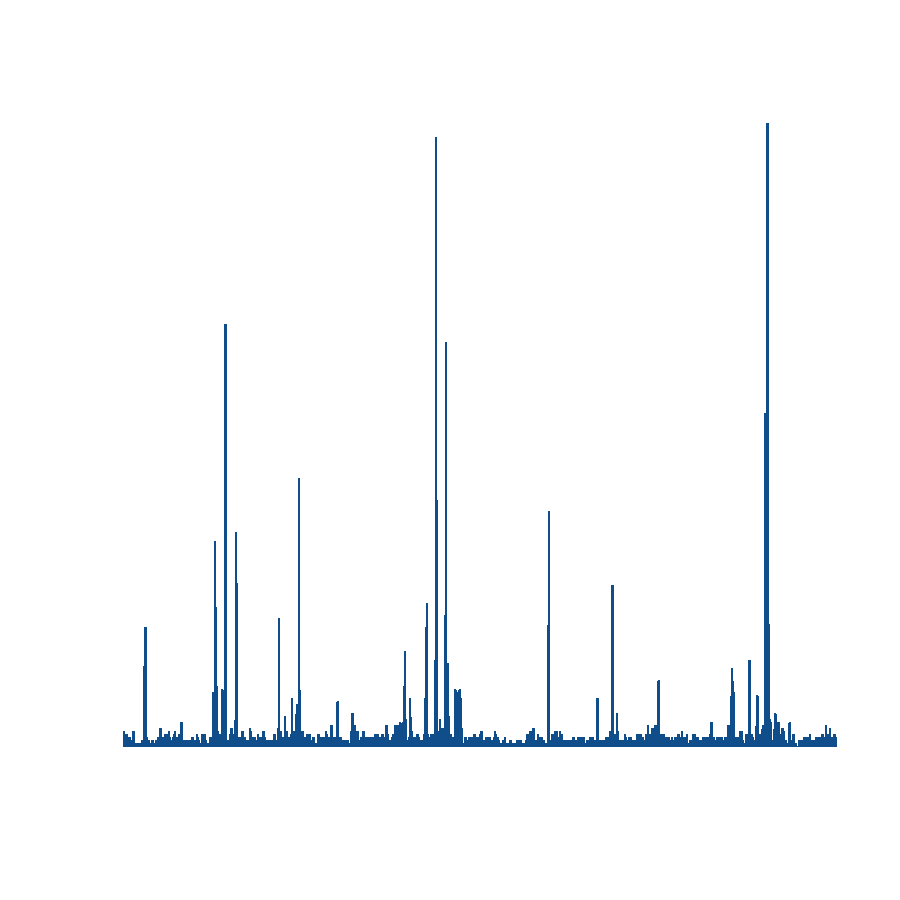
\includegraphics{Sushi-005}
\end{center}

To annotate the genome postion we use the 'labelgenome' function.  "n = 4" specifies the desired number of tickmarks.  And the scale is set to "Mb" (other options are "Kb" or "bp").

\begin{center}
\begin{Schunk}
\begin{Sinput}
> labelgenome(chrom,chromstart,chromend,n=4,scale="Mb")
\end{Sinput}
\end{Schunk}

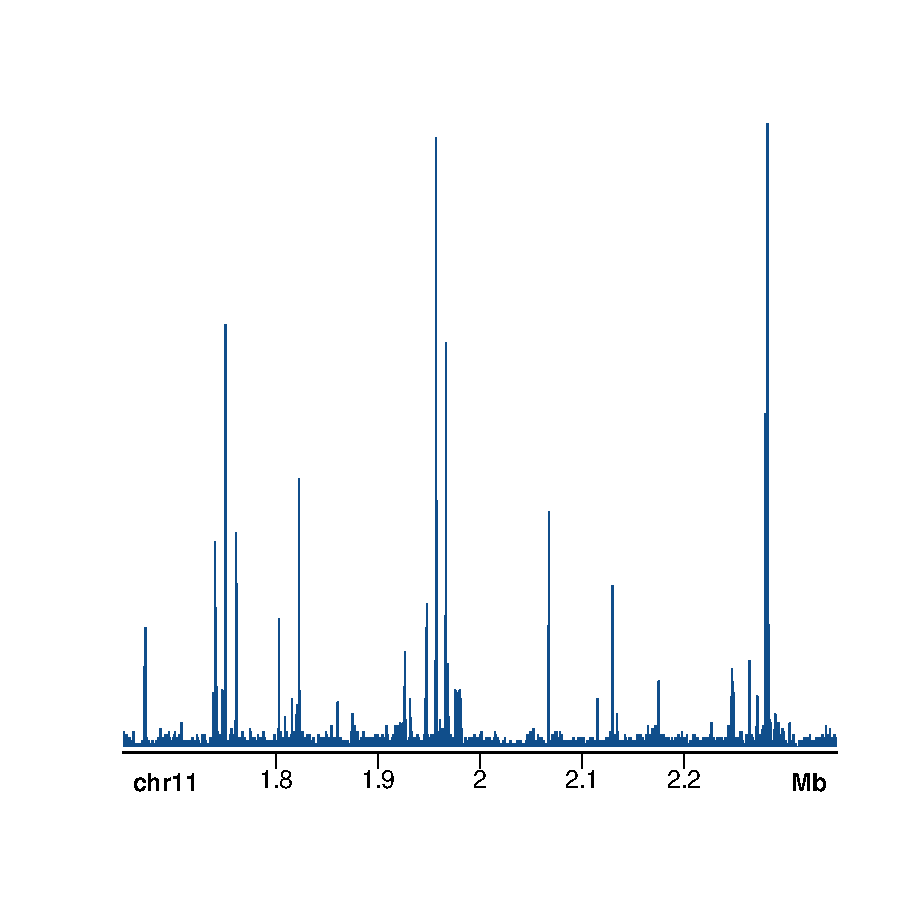
\includegraphics{Sushi-007}
\end{center}


The y-axis can be added using basic R functions 'mtext' and 'axis'.

\begin{center}

\begin{Schunk}
\begin{Sinput}
> mtext("Read Depth",side=2,line=1.75,cex=1,font=2)
> axis(side=2,las=2,tcl=.2)
\end{Sinput}
\end{Schunk}

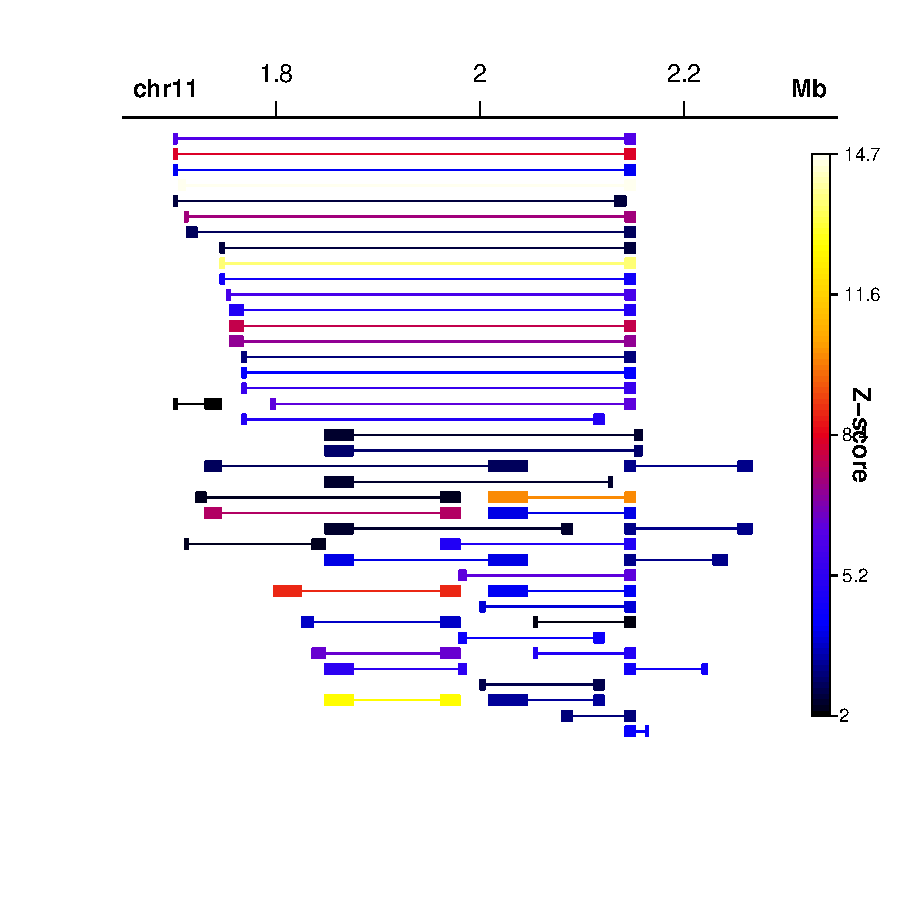
\includegraphics{Sushi-009}
\end{center}

Multiple bedgraph tracks can be plotted on the same plot by setting overlay=TRUE.  Transparencies can be added for easier viewing by adjusting the transcparency value.  The second plot can be rescaled to the maximum of the first plot by setting rescaleoverlay=TRUE.

\begin{center}
\begin{Schunk}
\begin{Sinput}
> chrom            = "chr11"
> chromstart       = 1955000
> chromend         = 1960000
> plotBedgraph(Sushi_ChIPSeq_CTCF.bedgraph,chrom,chromstart,chromend,
              transparency=.50,color="blue",linecol="blue")
> plotBedgraph(Sushi_DNaseI.bedgraph,chrom,chromstart,chromend,
              transparency=.50,color="#E5001B",overlay=TRUE,
              rescaleoverlay=TRUE)
> labelgenome(chrom,chromstart,chromend,n=3,scale="Kb")
\end{Sinput}
\end{Schunk}
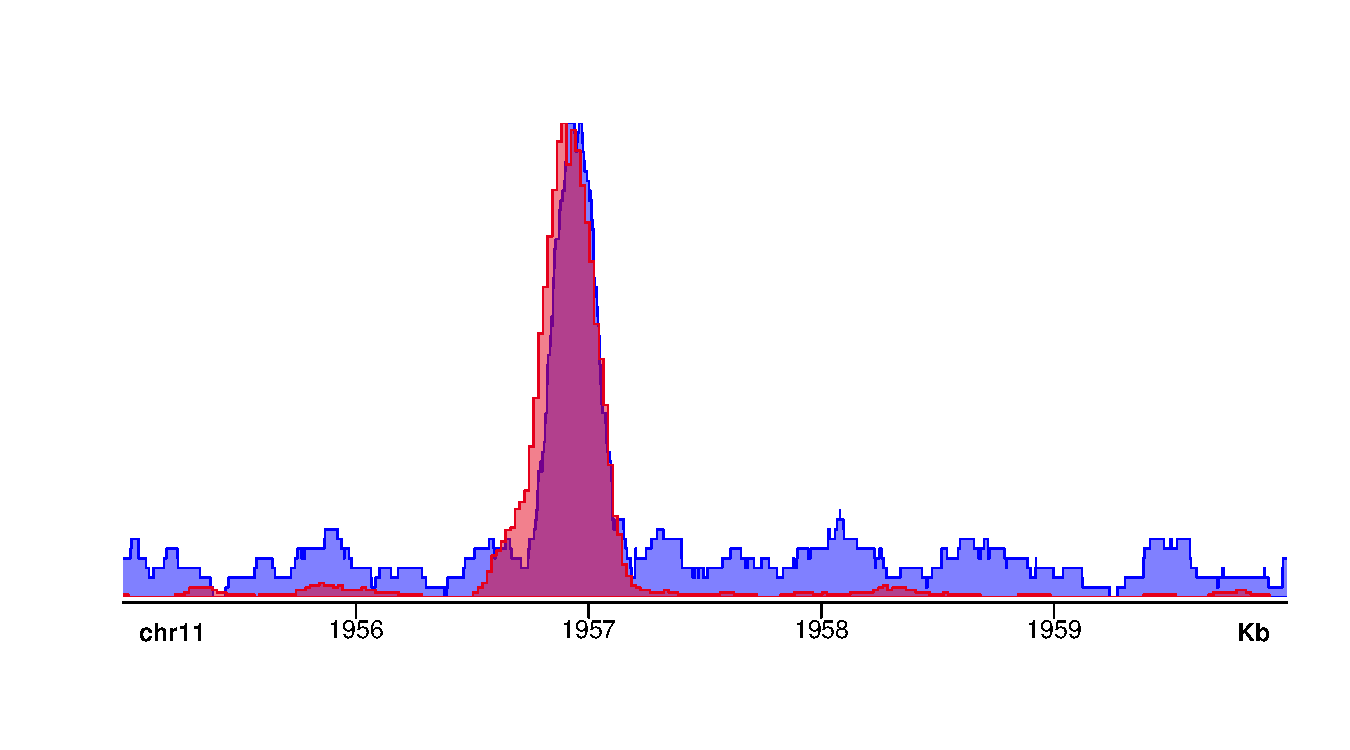
\includegraphics{Sushi-010}
\end{center}

Then we can use the base R function legend to add a legend to the plot.  First we need ot use the rgb function to add transparency to the colors in order to match out plot.

\begin{center}

\begin{Schunk}
\begin{Sinput}
> finalcolor1 = rgb(col2rgb("blue")[1],col2rgb("blue")[2],col2rgb("blue")[3],
                   alpha=.5 * 255,max = 255)
> finalcolor2 = rgb(col2rgb("#E5001B")[1],col2rgb("#E5001B")[2],col2rgb("#E5001B")[3],
                   alpha=.5 * 255,max = 255)
> legend("topright",inset=0.025,legend=c("DnaseI","ChIP-seq (CTCF)"),
        fill=c(finalcolor1,finalcolor2),border=c("blue","#E5001B"),text.font=2,
        cex=1.0)
\end{Sinput}
\end{Schunk}
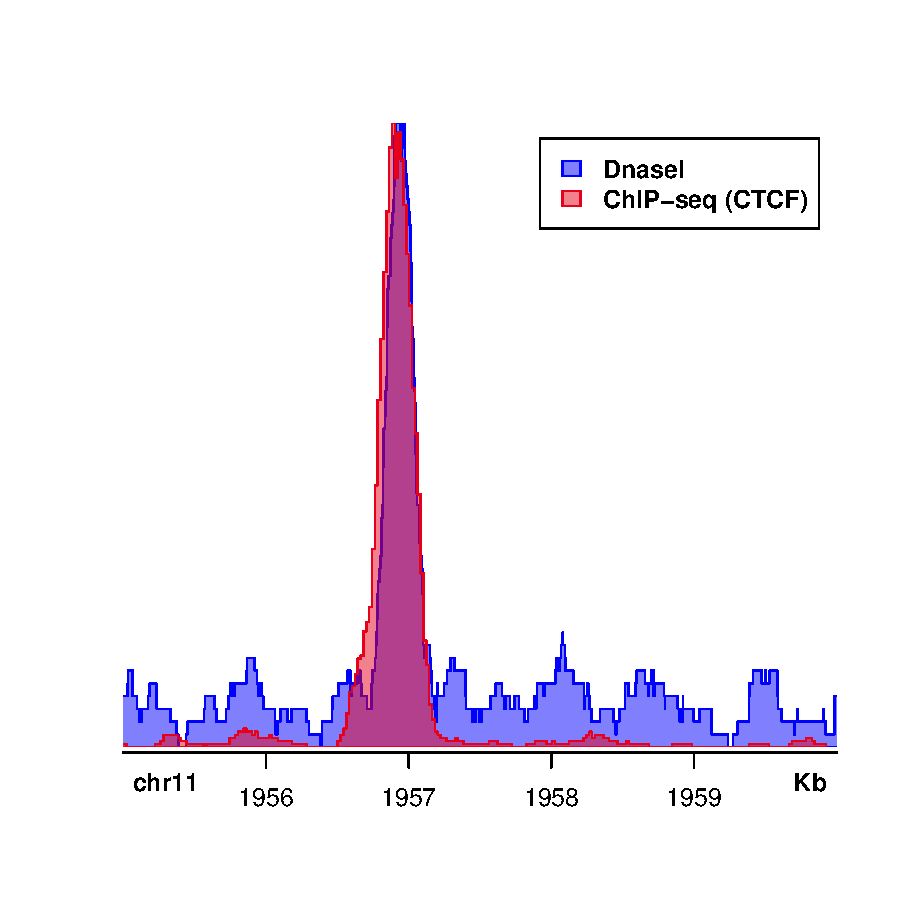
\includegraphics{Sushi-012}

\end{center}

Setting flip=TRUE is another method that can be used to compare tracks.  First, we will use mfrow to divided the plotting divice into two vertically stacked regions.

\begin{center}
\begin{Schunk}
\begin{Sinput}
> par(mfrow=c(2,1),mar=c(1,4,1,1))
\end{Sinput}
\end{Schunk}
\end{center}

Next, we plot the first plot.  We set the transparency of the plot to 0.5. We will also add the legend.

\begin{center}
\begin{Schunk}
\begin{Sinput}
> plotBedgraph(Sushi_ChIPSeq_CTCF.bedgraph,chrom,chromstart,chromend,transparency=.50,
              color="blue",linecol="blue")
> axis(side=2,las=2,tcl=.2)
> mtext("Read Depth",side=2,line=1.75,cex=1,font=2)
> legend("topright",inset=0.025,legend=c("DnaseI","ChIP-seq (CTCF)"),
        fill=c(finalcolor1,finalcolor2),border=c("blue","#E5001B"),text.font=2)
\end{Sinput}
\end{Schunk}
\end{center}


\begin{center}
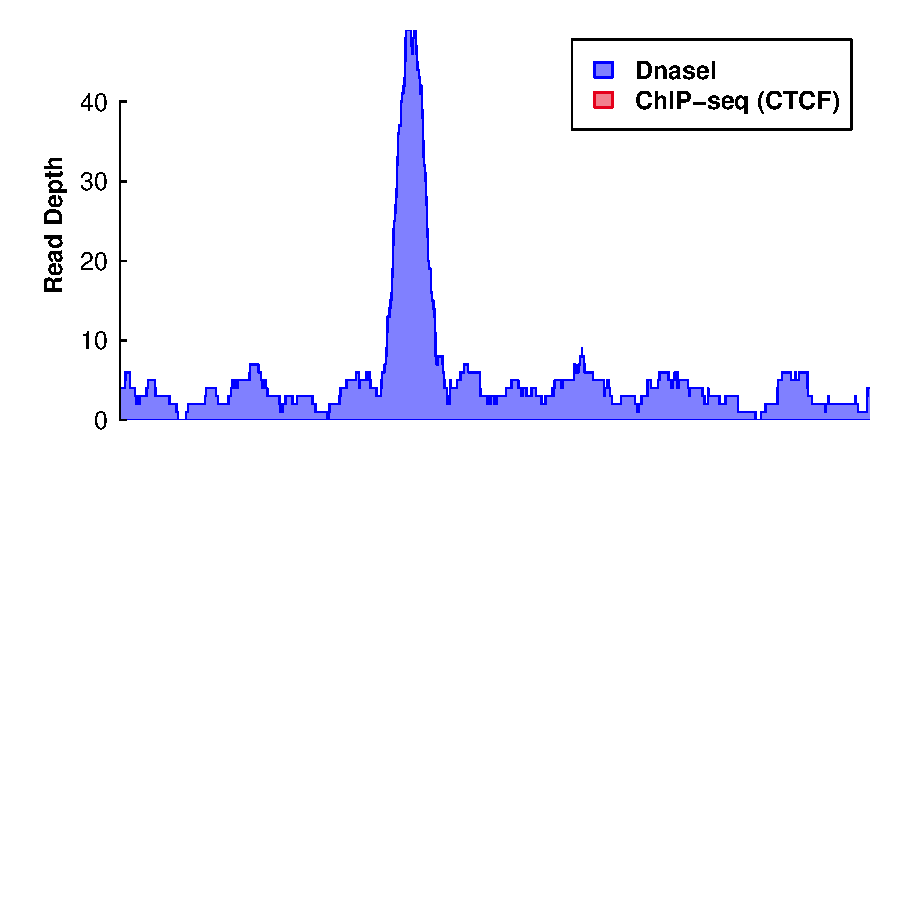
\includegraphics{Sushi-015}
\end{center}

Finally, we add the second plot with flip=TRUE.  We will also label the x-axis using labelgenome and label the y-axis using mtext and axis.

\begin{center}
\begin{Schunk}
\begin{Sinput}
> plotBedgraph(Sushi_DNaseI.bedgraph,chrom,chromstart,chromend,transparency=.50,
              flip=TRUE,color="#E5001B")
> labelgenome(chrom,chromstart,chromend,side=3,n=3,scale="Kb")
> axis(side=2,las=2,tcl=.2,at=pretty(par("yaxp")[c(1,2)]),
              labels=-1*pretty(par("yaxp")[c(1,2)]))
> mtext("Read Depth",side=2,line=1.75,cex=1,font=2)
\end{Sinput}
\end{Schunk}
\end{center}


\begin{center}
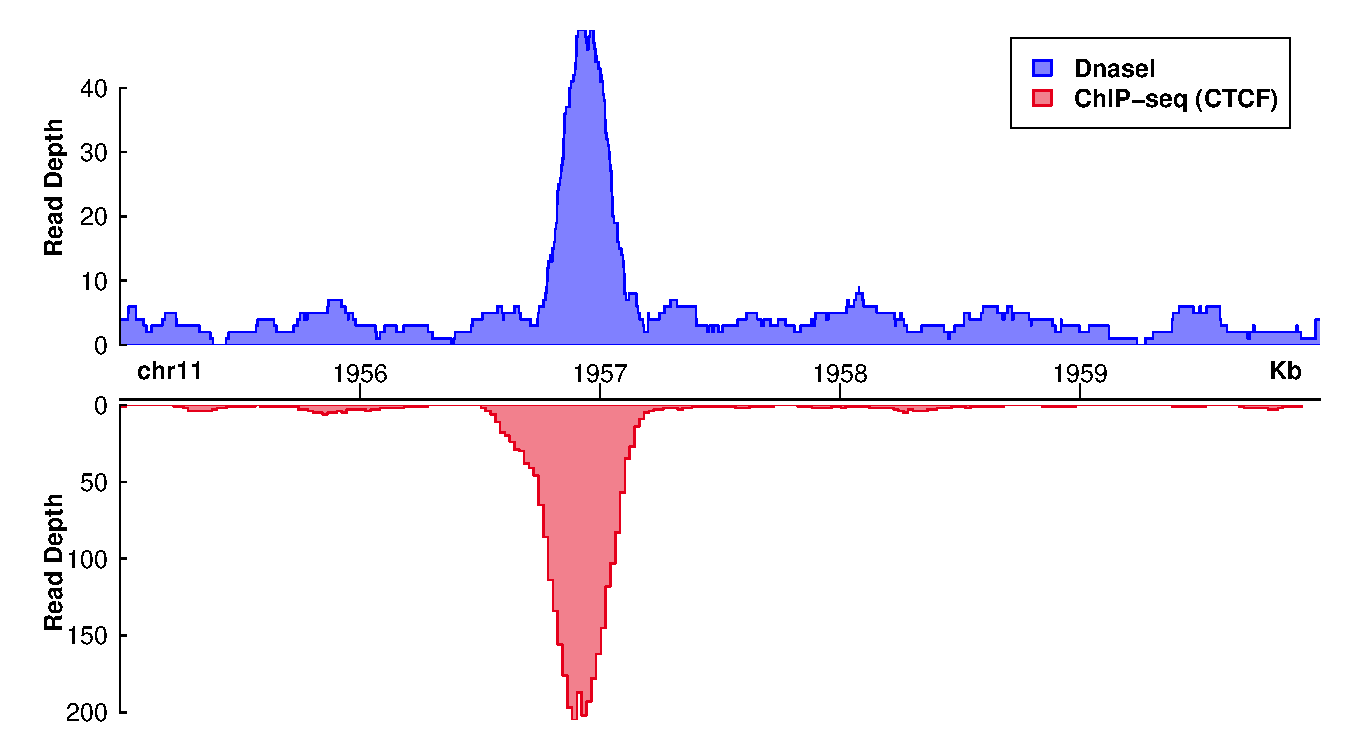
\includegraphics{Sushi-017}
\end{center}


\section{plotHiC}

HiC interaction plots can be plotted given an interaction matrix in which row and column names are genomic coordiates and matrix values are some tye of interaction score.

\begin{Schunk}
\begin{Sinput}
>   Sushi_HiC.matrix[100:105,100:105]
\end{Sinput}
\begin{Soutput}
          3980000   4020000   4060000  4100000   4140000   4180000
3980000  0.000000 50.087965 49.689032 22.89760  7.438259  2.219527
4020000 50.087965 40.469337 33.922805 24.07214 12.652542  3.620466
4060000 49.689032 33.922805 26.998026 30.17873 21.879022  6.850893
4100000 22.897599 24.072145 30.178735 54.47335 48.570924 11.379299
4140000  7.438259 12.652542 21.879022 48.57092 45.265394 26.369969
4180000  2.219527  3.620466  6.850893 11.37930 26.369969 11.413106
\end{Soutput}
\end{Schunk}

The 'plotHiC' function is used to plot the data while the 'labelgenome' function is used to add the genome labels to the x-axis.  'plotHiC' returns an object indicating the color palette and data range that can be fed into 'addlegend' to create a legend.

\begin{center}

\begin{Schunk}
\begin{Sinput}
> chrom            = "chr11"
> chromstart       = 500000
> chromend         = 5050000
> phic = plotHic(Sushi_HiC.matrix,chrom,chromstart,chromend,max_y = 20,
                zrange=c(0,28),palette=SushiColors("fire"))
> addlegend(phic[[1]],palette=phic[[2]],title="score",side="right",bottominset=0.4,
           topinset=0,xoffset=-.035,labelside="left",width=0.025,title.offset=0.035)
> labelgenome(chrom,chromstart,chromend,n=4,scale="Mb",edgeblankfraction=0.20)
\end{Sinput}
\end{Schunk}
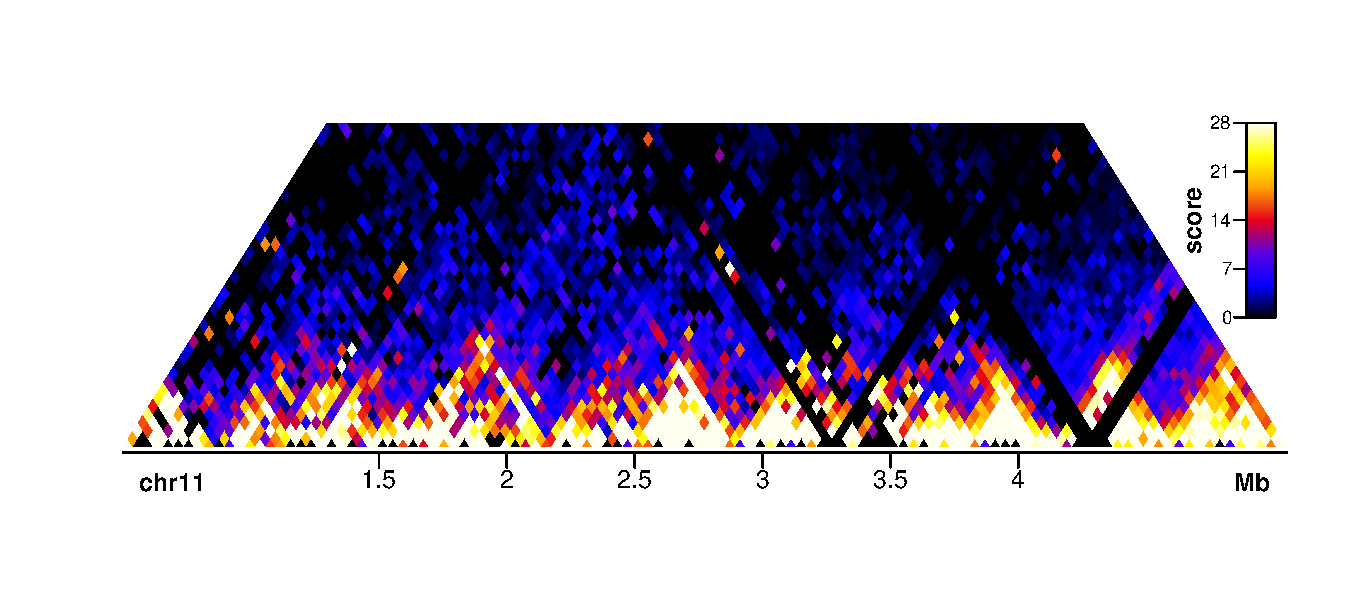
\includegraphics{Sushi-019}
\end{center}

plotHic has a number of customizable options.  The plot can be flipped over the x-axis by setting flip = TRUE.  The color palette can be changed by the palette argument. 

addlegend also has customizable features.  The legend can be moved to the left side of the plot by setting side = "left" and the labeling canbe moved to the right side of the lenged buy setting labelside = "right".  The vertical position of the legend can be adjusted by changing the topinset and bottominset.

Finally, the x-axis label can be moved to the top of the plot by setting side = 3 in the labelgenome function.

\begin{center}

\begin{Schunk}
\begin{Sinput}
> chrom            = "chr11"
> chromstart       = 500000
> chromend         = 5050000
> phic = plotHic(Sushi_HiC.matrix,chrom,chromstart,chromend,max_y = 20,
                zrange=c(0,28),flip=TRUE,palette=topo.colors)
> addlegend(phic[[1]],palette=phic[[2]],title="score",side="left",bottominset=0.1,
           topinset=0.5,xoffset=-.035,labelside="right",width=0.025,title.offset=0.035)
> labelgenome(chrom,chromstart,chromend,side=3,n=4,scale="Mb",edgeblankfraction=0.20)
\end{Sinput}
\end{Schunk}
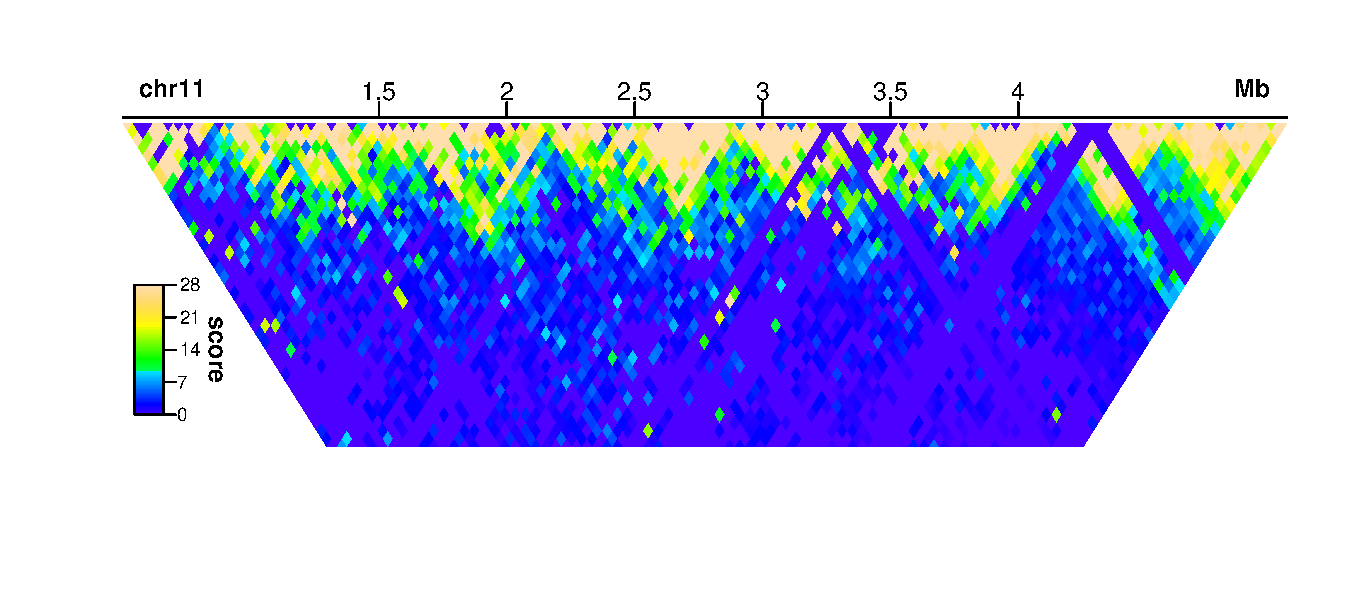
\includegraphics{Sushi-020}
\end{center}



\section{plotBedpe}

plotBedpe allows for data in bedpe format to be plotted in multiple fashions.  To illustrate this we will use 5C data formatted in the following way.

\begin{Schunk}
\begin{Sinput}
>   head(Sushi_5C.bedpe)
\end{Sinput}
\begin{Soutput}
  chrom1    start1      end1 chrom2    start2      end2 name    score strand1
1   chr2 234208447 234223064   chr2 234156762 234159135   NA 44.39862       .
2  chr15  41711734  41718116  chr15  41802421  41808201   NA 20.62534       .
3  chr11  64172456  64183193  chr11  64068878  64079209   NA 16.91630       .
4   chr2 234208447 234223064   chr2 234163674 234170252   NA 12.34501       .
5   chr6  41755186  41769245   chr6  41435903  41452283   NA 11.63480       .
6  chr11  64159283  64172456  chr11  64068878  64079209   NA 11.13098       .
  strand2 samplenumber
1       .            1
2       .            1
3       .            1
4       .            1
5       .            1
6       .            1
\end{Soutput}
\end{Schunk}

plotBedpe can plot bedpe as arches.  The height, linewidth, and color of each arch can be scaled to represent different aspects of the data.  Here the height of the arches represents the Z-score of the 5C interaction, the color represents the cell line each interaction was detected in, and the line widths are kept constant.

\begin{center}

\begin{Schunk}
\begin{Sinput}
> chrom            = "chr11"
> chromstart       = 1650000
> chromend         = 2350000
> pbpe = plotbedpe(Sushi_5C.bedpe,chrom,chromstart,chromend,heights = Sushi_5C.bedpe$score,
                  plottype="loops",colorby=Sushi_5C.bedpe$samplenumber,
                  colorbycol=SushiColors("three"))
> labelgenome(chrom, chromstart,chromend,n=3,scale="Mb")
> legend("topright",inset =0.01,legend=c("K562","HeLa","GM12878"),
        col=SushiColors("three")(3),pch=19,bty='n',text.font=2)
> axis(side=2,las=2,tcl=.2)
> mtext("Z-score",side=2,line=1.75,cex=.75,font=2)
\end{Sinput}
\end{Schunk}
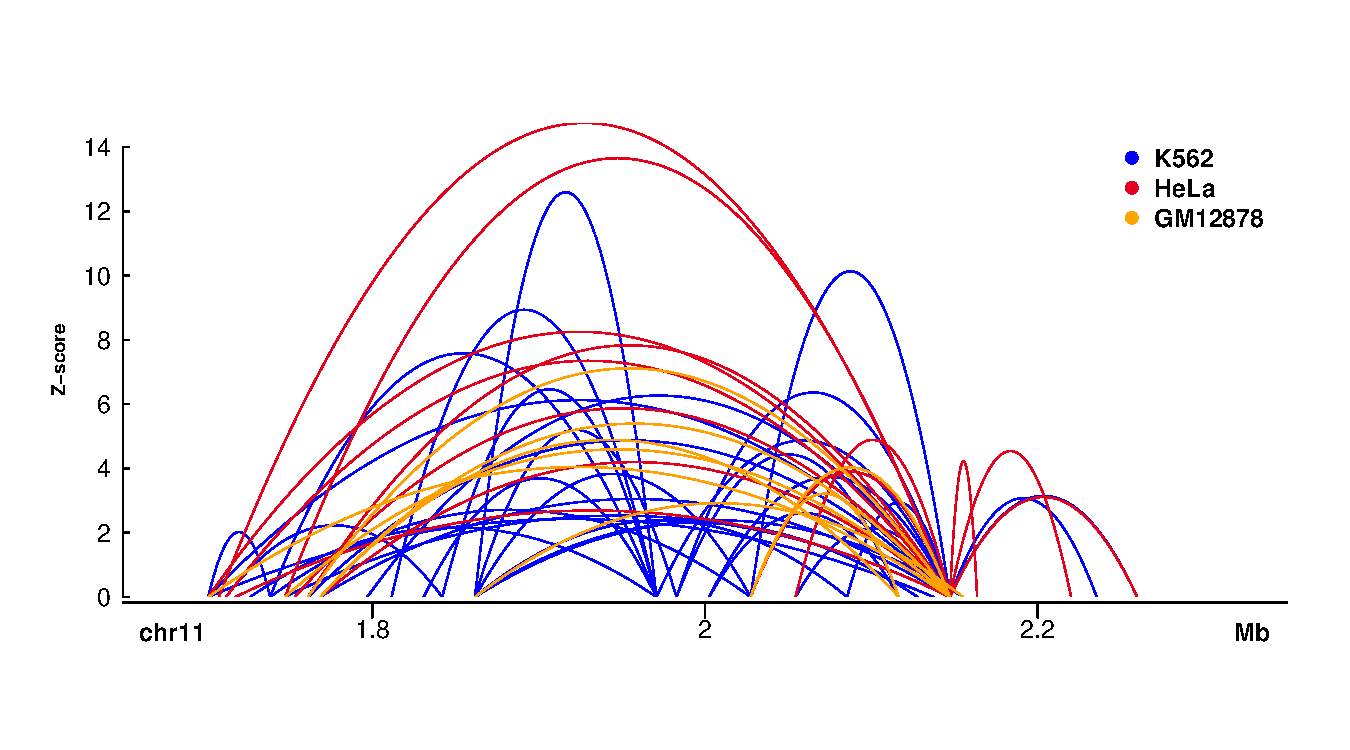
\includegraphics{Sushi-022}
\end{center}

The plot can be flipped over the x-axis by setting flip = TRUE,  Bedpe elements can be represented by boxes and straight lines by setting plottype = "lines".  And colors can be used to represent Z-scores by setting colorby = "Sushi_5C.bedpe$score". 

\begin{center}

\begin{Schunk}
\begin{Sinput}
> chrom            = "chr11"
> chromstart       = 1650000
> chromend         = 2350000
> pbpe = plotbedpe(Sushi_5C.bedpe,chrom,chromstart,chromend,flip=TRUE,
                  plottype="lines",colorby=Sushi_5C.bedpe$score,
                  colorbycol=SushiColors("firedark"))
> labelgenome(chrom, chromstart,chromend,side=3,n=3,scale="Mb")
> addlegend(pbpe[[1]],palette=pbpe[[2]],title="Z-score",side="right",bottominset=0.05,
           topinset=0.05,xoffset=-.035,labelside="right",width=0.025,title.offset=0.045)
\end{Sinput}
\end{Schunk}
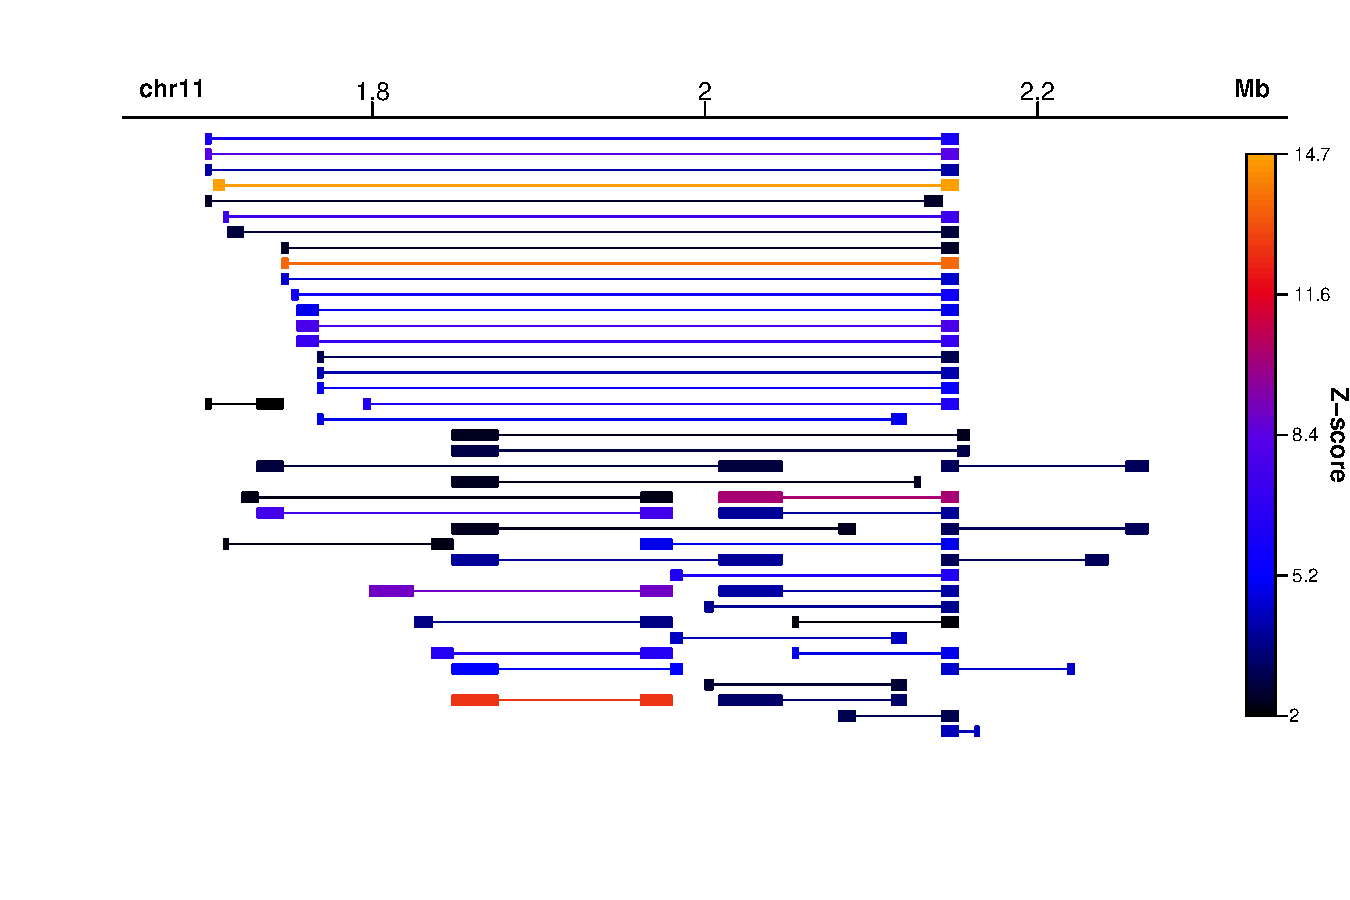
\includegraphics{Sushi-023}

\end{center}


\section{plotBed}

plotBed provides multiple different ways to represent genomic data stored in bed format.  Below are the first six lines of a bed file detailing reads from Pol2 ChIP-Seq analysis of K562 cells.

\begin{Schunk}
\begin{Sinput}
>   head(Sushi_ChIPSeq_pol2.bed)
\end{Sinput}
\begin{Soutput}
  chrom   start     end                        name score strand
1 chr11 2280543 2280570 GGGCTCTCTCCGGCTTCCCTGTCCCGT    63     -1
2 chr11 2288946 2288973 CCTTCCCATCCGCAGGGGCACCACATG  1000     -1
3 chr11 2272471 2272498 TGGGCATCAGTCAGGCTCCTTCCCCAG  1000     -1
4 chr11 2288939 2288966 ATCCGCAGGGGCACCACATGAGTCACC  1000     -1
5 chr11 2281534 2281561 TGTCCTAGTGACAAGTGGCCGGACTTG   250     -1
6 chr11 2286805 2286832 GGTGAGGGCCAGCAGCTCCCTGGGGGG   250      1
\end{Soutput}
\end{Schunk}

Leaving row set to 'auto' provide a pile-sup style plot.  Here the colorby argument is used to color the bed elements by the strand.

\begin{center}
\begin{Schunk}
\begin{Sinput}
> chrom            = "chr11"
> chromstart       = 2281200
> chromend         = 2282200
> plotBed(beddata    = Sushi_ChIPSeq_pol2.bed,chrom = chrom,chromstart = chromstart,
         chromend =chromend,colorby    = Sushi_ChIPSeq_pol2.bed$strand,
         colorbycol = SushiColors("two"),row  = "auto",wiggle=0.001)
> labelgenome(chrom,chromstart,chromend,n=2,scale="Kb")
> legend("topright",inset=0,legend=c("reverse","forward"),fill=SushiColors("two")(2),
        border=SushiColors("two")(2),text.font=2,cex=0.75)
\end{Sinput}
\end{Schunk}
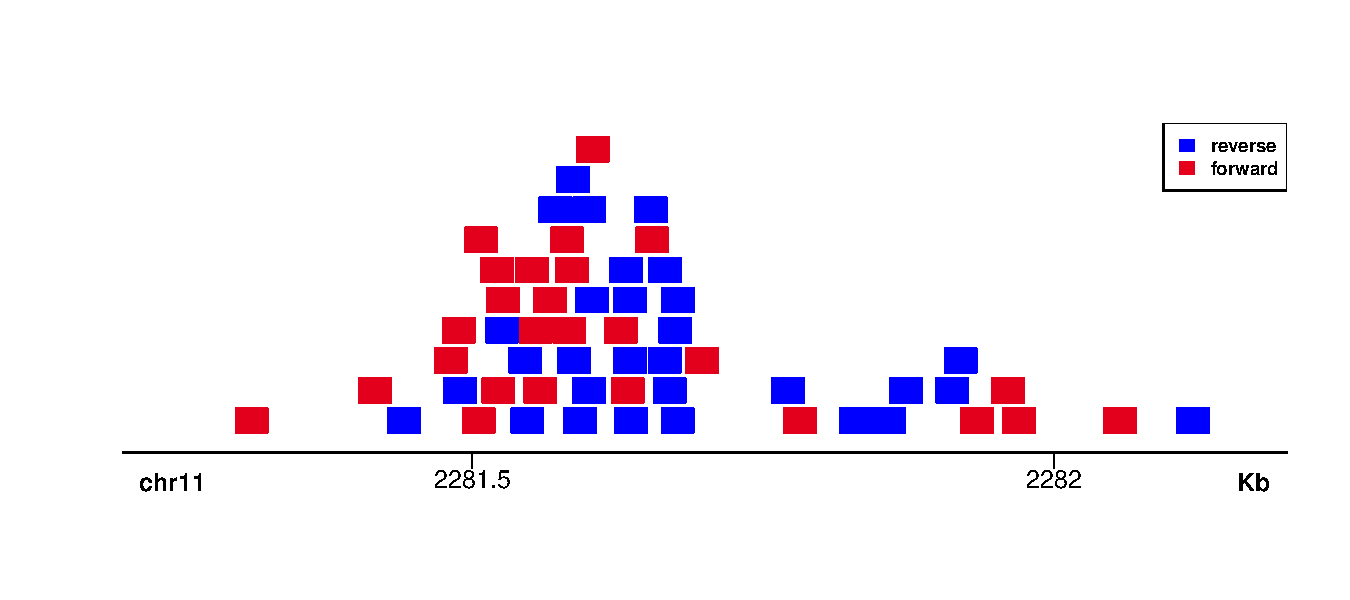
\includegraphics{Sushi-025}
\end{center}

Setting splitstrand = TRUE plots reads from different strands in two separate vertical regions.

\begin{center}
\begin{Schunk}
\begin{Sinput}
> chrom            = "chr11"
> chromstart       = 2281200
> chromend         = 2282200
> plotBed(beddata    = Sushi_ChIPSeq_pol2.bed,chrom = chrom,chromstart = chromstart,
         chromend =chromend,colorby    = Sushi_ChIPSeq_pol2.bed$strand,
         colorbycol = SushiColors("two"),row  = "auto",wiggle=0.001,splitstrand=TRUE)
> labelgenome(chrom,chromstart,chromend,n=2,scale="Kb")
> legend("topright",inset=0,legend=c("reverse","forward"),fill=SushiColors("two")(2),
        border=SushiColors("two")(2),text.font=2,cex=0.75)
\end{Sinput}
\end{Schunk}
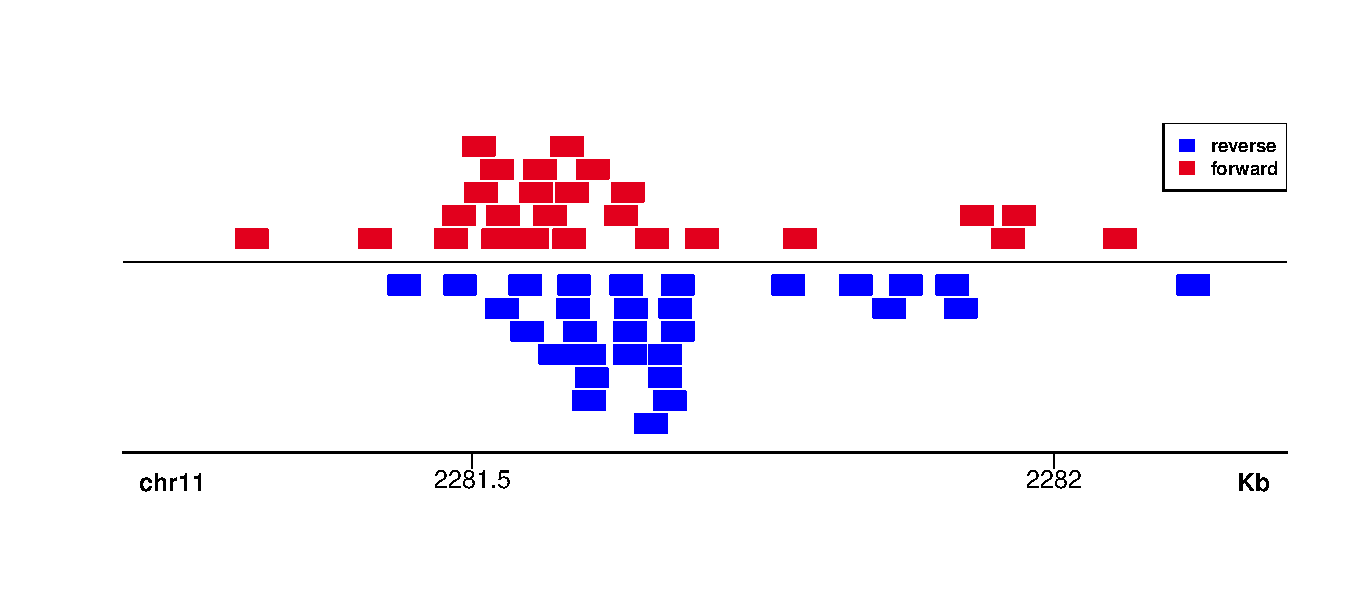
\includegraphics{Sushi-026}
\end{center}

By providing row and color information plotBed can be used to compare bed elements from different samples by plotting them on different rows.  we can use the Sushi function maptocolors to assign a different color to each row.

\begin{center}
\begin{Schunk}
\begin{Sinput}
> chrom            = "chr15"
> chromstart      = 72800000
> chromend         = 73100000
> Sushi_ChIPSeq_severalfactors.bed$color = 
         maptocolors(Sushi_ChIPSeq_severalfactors.bed$row,
         col=SushiColors("firenowhite"))
> plotBed(beddata    = Sushi_ChIPSeq_severalfactors.bed,chrom = chrom,
         chromstart = chromstart,chromend =chromend,
         rownumber  = Sushi_ChIPSeq_severalfactors.bed$row, type = "circles",
         color=Sushi_ChIPSeq_severalfactors.bed$color,row="given",
         plotbg="grey95",rowlabels=unique(Sushi_ChIPSeq_severalfactors.bed$name),
         rowlabelcol=unique(Sushi_ChIPSeq_severalfactors.bed$color),rowlabelcex=0.75)
> labelgenome(chrom,chromstart,chromend,n=3,scale="Mb")
> mtext("ChIP-seq",side=3, adj=-0.065,line=0.5,font=2)
\end{Sinput}
\end{Schunk}
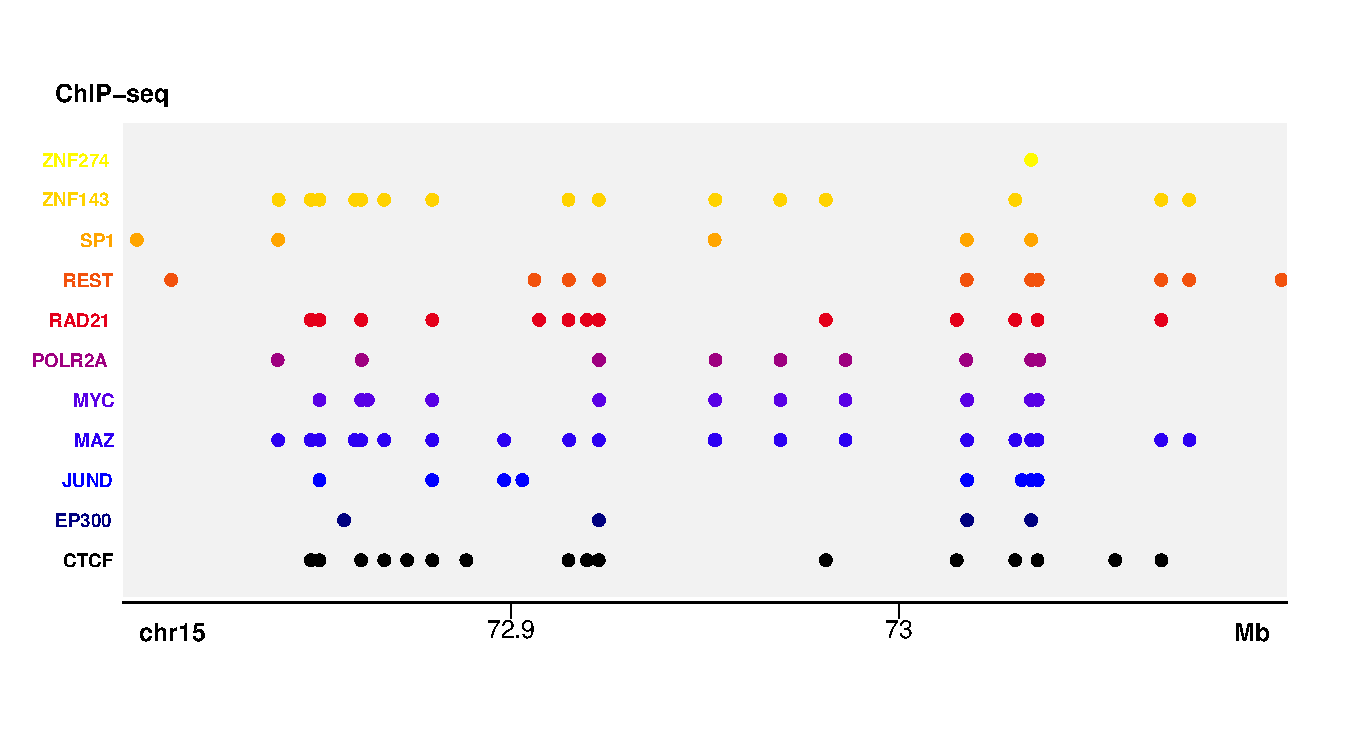
\includegraphics{Sushi-027}
\end{center}

The bed elements can also be represented by rectangles that depict the actual width of each bed element.

\begin{center}
\begin{Schunk}
\begin{Sinput}
> chrom            = "chr15"
> chromstart       = 72800000
> chromend         = 73100000
> Sushi_ChIPSeq_severalfactors.bed$color = 
         maptocolors(Sushi_ChIPSeq_severalfactors.bed$row,
         col=SushiColors("firenowhite"))
> plotBed(beddata    = Sushi_ChIPSeq_severalfactors.bed,chrom = chrom,
         chromstart = chromstart,chromend =chromend,
         rownumber  = Sushi_ChIPSeq_severalfactors.bed$row, type = "region",
         color=Sushi_ChIPSeq_severalfactors.bed$color,row="given",
         plotbg="grey95",rowlabels=unique(Sushi_ChIPSeq_severalfactors.bed$name),
         rowlabelcol=unique(Sushi_ChIPSeq_severalfactors.bed$color),rowlabelcex=0.75)
> labelgenome(chrom,chromstart,chromend,n=3,scale="Mb")
> mtext("ChIP-seq",side=3, adj=-0.065,line=0.5,font=2)
\end{Sinput}
\end{Schunk}
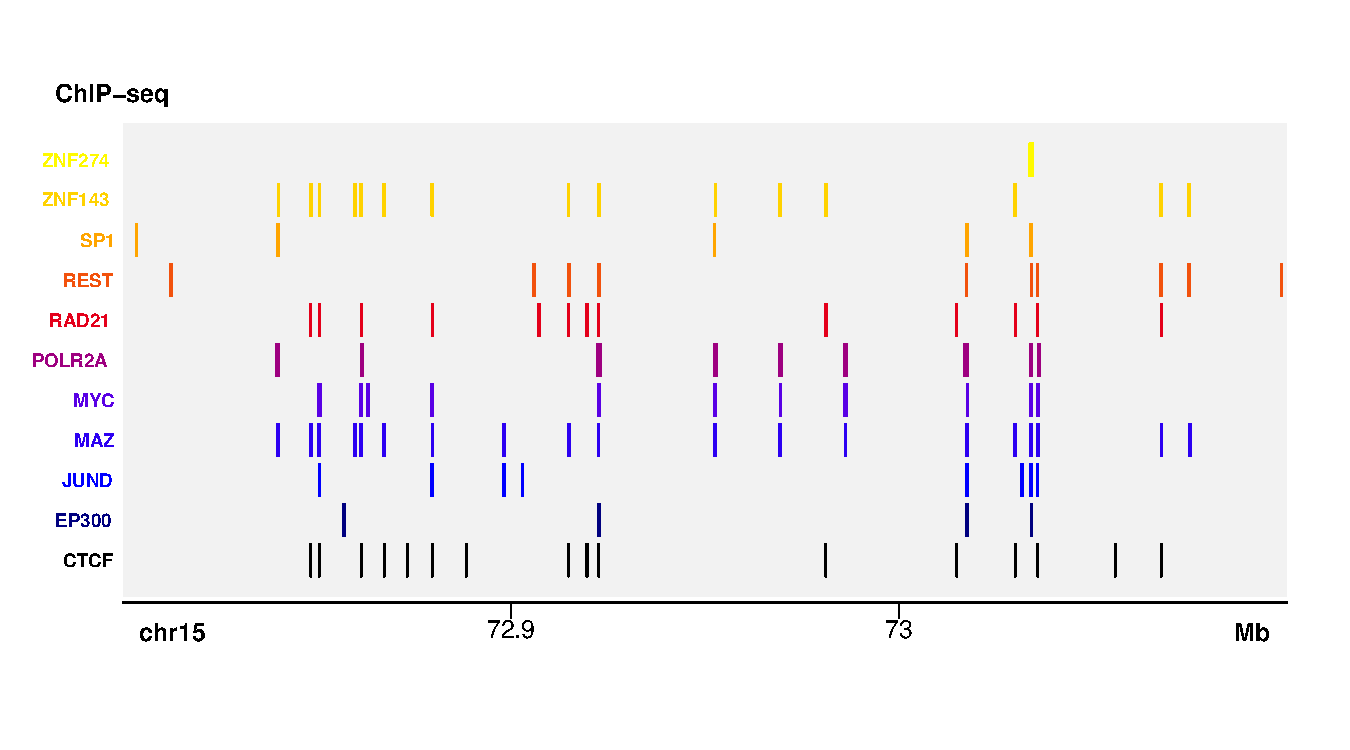
\includegraphics{Sushi-028}
\end{center}

plotBed can also be used to plot heatmaps representing the density of bed elements.  A plot depicting gene density is shown below.

\begin{center}
\begin{Schunk}
\begin{Sinput}
> par(mar=c(3,1,1,1))
> chrom            = "chr15"
> chromstart       = 60000000
> chromend         = 80000000
> chrom_biomart    = gsub("chr","",chrom)
> mart=useMart(host='may2009.archive.ensembl.org', biomart='ENSEMBL_MART_ENSEMBL', 
              dataset='hsapiens_gene_ensembl')
> geneinfobed = getBM(attributes = c("chromosome_name","start_position","end_position"),
                     filters= c("chromosome_name","start","end"),
                     values=list(chrom_biomart,chromstart,chromend),mart=mart)
> geneinfobed[,1] = paste("chr",geneinfobed[,1],sep="")
> plotBed(beddata = geneinfobed[!duplicated(geneinfobed),],chrom = chrom,
         chromstart = chromstart,chromend =chromend,row='supplied',
         palettes = list(heat.colors), type = "density")
> labelgenome(chrom, chromstart, chromend,  n=4,scale="Mb",edgeblankfraction=0.10)
> mtext("Gene Density",side=3, adj=0,line=0.20,font=2)
\end{Sinput}
\end{Schunk}
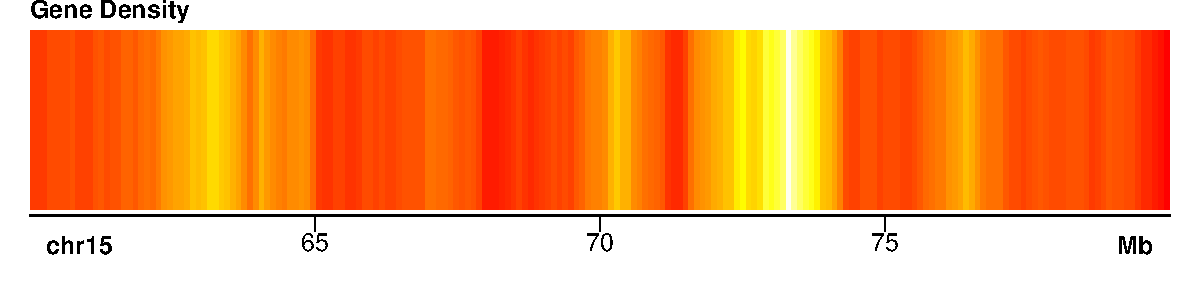
\includegraphics{Sushi-029}
\end{center}



\section{plotManhattan}

Manhattan plots can be plotted given SNPS and significance values in bed format.

\begin{Schunk}
\begin{Sinput}
>   head(Sushi_GWAS.bed)
\end{Sinput}
\begin{Soutput}
  chr.hg18 pos.hg18 pos.hg18.1       rsid pval.GC.DBP V6
1     chr1  1695996    1695996  rs6603811    0.003110  .
2     chr1  1696020    1696020  rs7531583    0.000824  .
3     chr1  1698661    1698661 rs12044597    0.001280  .
4     chr1  1711339    1711339  rs2272908    0.001510  .
5     chr1  1712792    1712792  rs3737628    0.001490  .
6     chr1  1736016    1736016 rs12408690    0.004000  .
\end{Soutput}
\end{Schunk}

The 'plotManhattan' function is used to plot the data while the 'labelgenome' function is used to add the genome labels to the x-axis.

\begin{center}

\begin{Schunk}
\begin{Sinput}
> plotManhattan(bedfile=Sushi_GWAS.bed,pvalues=Sushi_GWAS.bed[,5],col=SushiColors("firenowhite"),
                 genome=Sushi_hg18_genome,cex=0.75)
> labelgenome(genome=Sushi_hg18_genome,n=4,scale="Mb",edgeblankfraction=0.20,cex.axis=.5)
> axis(side=2,las=2,tcl=.2)
> mtext("log10(P)",side=2,line=1.75,cex=1,font=2)
> mtext("chromosome",side=1,line=1.75,cex=1,font=2)
\end{Sinput}
\end{Schunk}
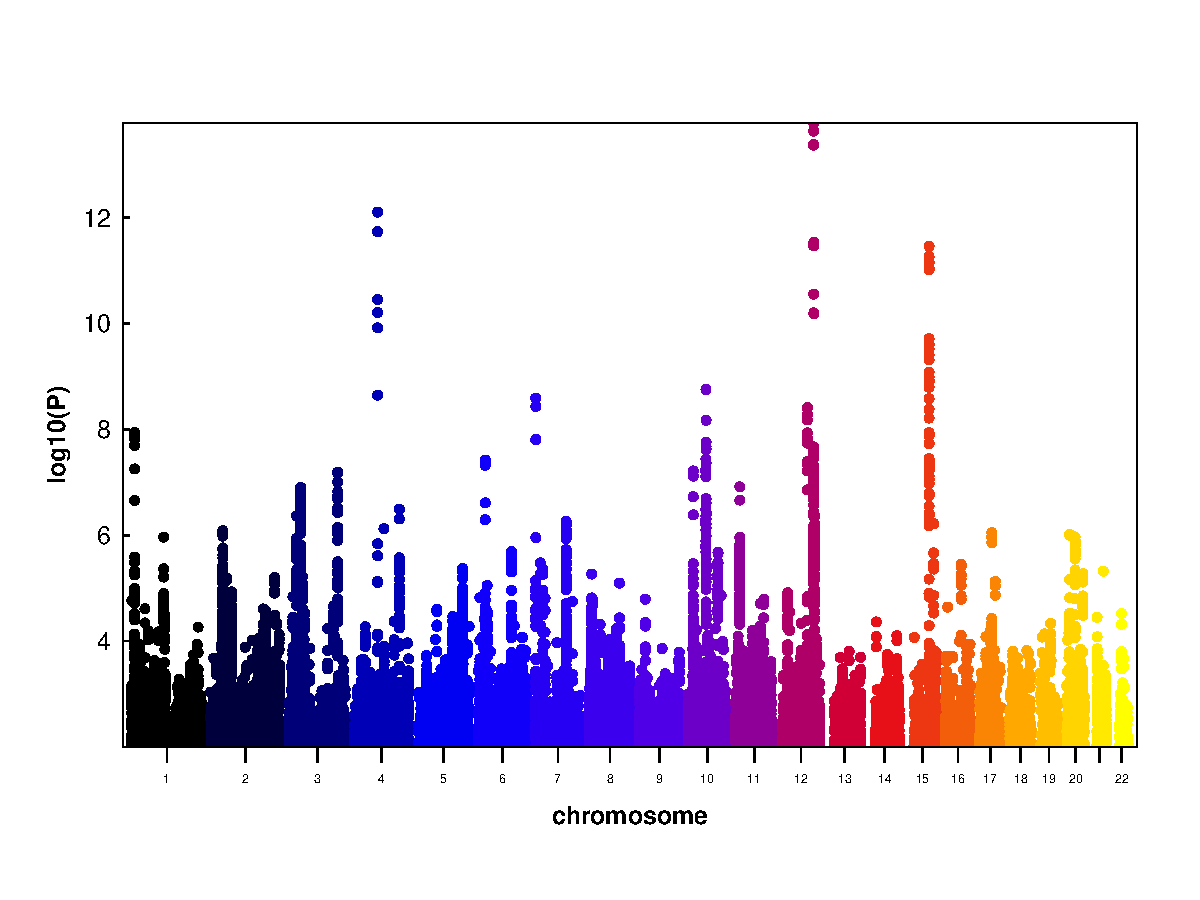
\includegraphics{Sushi-031}
\end{center}














\section{Creating Multi-panel Sushi Plots (with zoom functions) }

A critical characteristic of the Sushi package is its ability to create highly customizable, publication ready, multipanel figures.  Here, we will create a basic three panel figure and demonstrate how the zoom functions work (zoomsregion and zoombox).  To illustrate these feature we will use the plotBedgrpah function to plot bedgrpah data representing a DNaseI hypersensitivity experiment in K562 cells.

In order to make a multipanel figure we will use the R function layout.  Layout divides the device into rows and columns accoriding to a matrix you provide.  The matrix also tells it which plots will appear on which parts of the plotting device.  Below we make a 2 by matrix.  The entire top row will be used to plot the first plot while the bottom row with contain two plots.  For more info on layout try ?layout.

\begin{Schunk}
\begin{Sinput}
> layout(matrix(c(1,1,2,3),2, 2, byrow = TRUE))
> par(mar=c(3,4,1,1))
\end{Sinput}
\end{Schunk}

Next we will add the first plot

\begin{Schunk}
\begin{Sinput}
> chrom            = "chr11"
> chromstart       = 1900000
> chromend         = 2350000
> plotBedgraph(Sushi_DNaseI.bedgraph,chrom,chromstart=chromstart,chromend=chromend,
              color="#5900E5")
> labelgenome(chrom,chromstart=chromstart,chromend=chromend,n=4,scale="Mb")
> mtext("Read Depth",side=2,line=1.75,cex=1,font=2)
> axis(side=2,las=2,tcl=.2)
\end{Sinput}
\end{Schunk}


\begin{center}
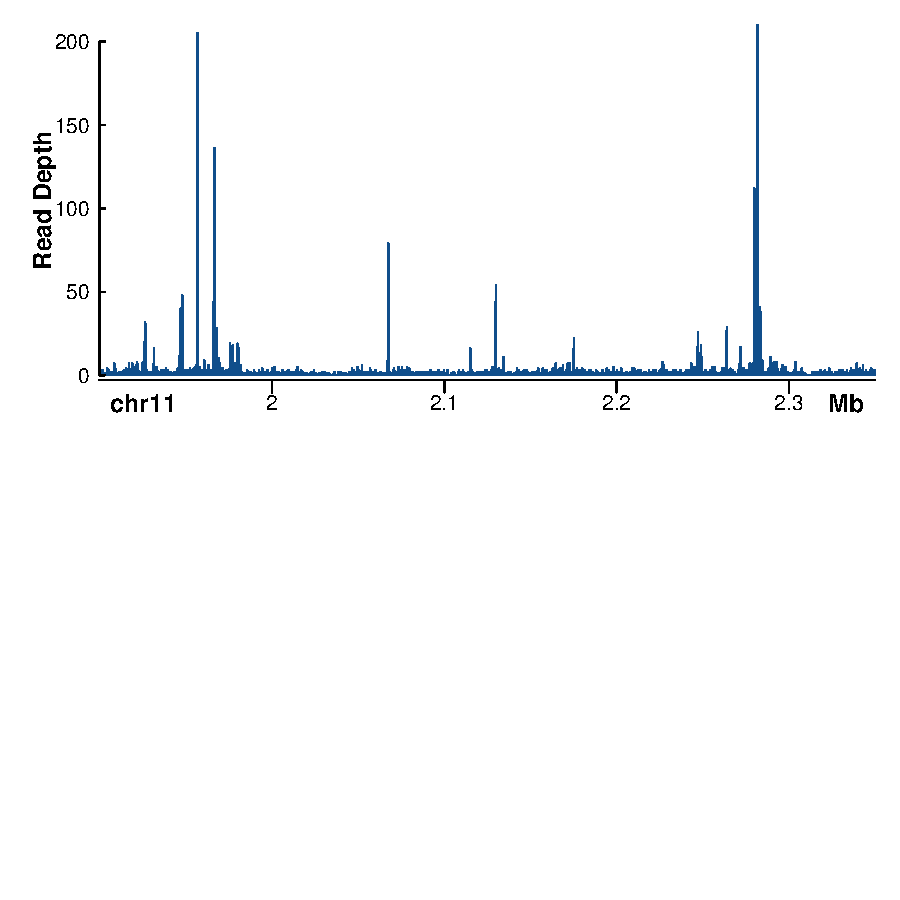
\includegraphics{Sushi-034}
\end{center}

Next we will add the zoom regions using the function 'zoomsregion'.  The argument 'offsets' is used to precisely position the left and right edges of the widest part of the zoom.

\begin{Schunk}
\begin{Sinput}
> zoomregion1      = c(1955000,1960000)
> zoomregion2      = c(2279000,2284000)
> zoomsregion(zoomregion1,extend=c(0.01,0.13),wideextend=0.05,offsets=c(0,0.580))
> zoomsregion(zoomregion2,extend=c(0.01,0.13),wideextend=0.05,offsets=c(0.580,0))
\end{Sinput}
\end{Schunk}

\begin{center}
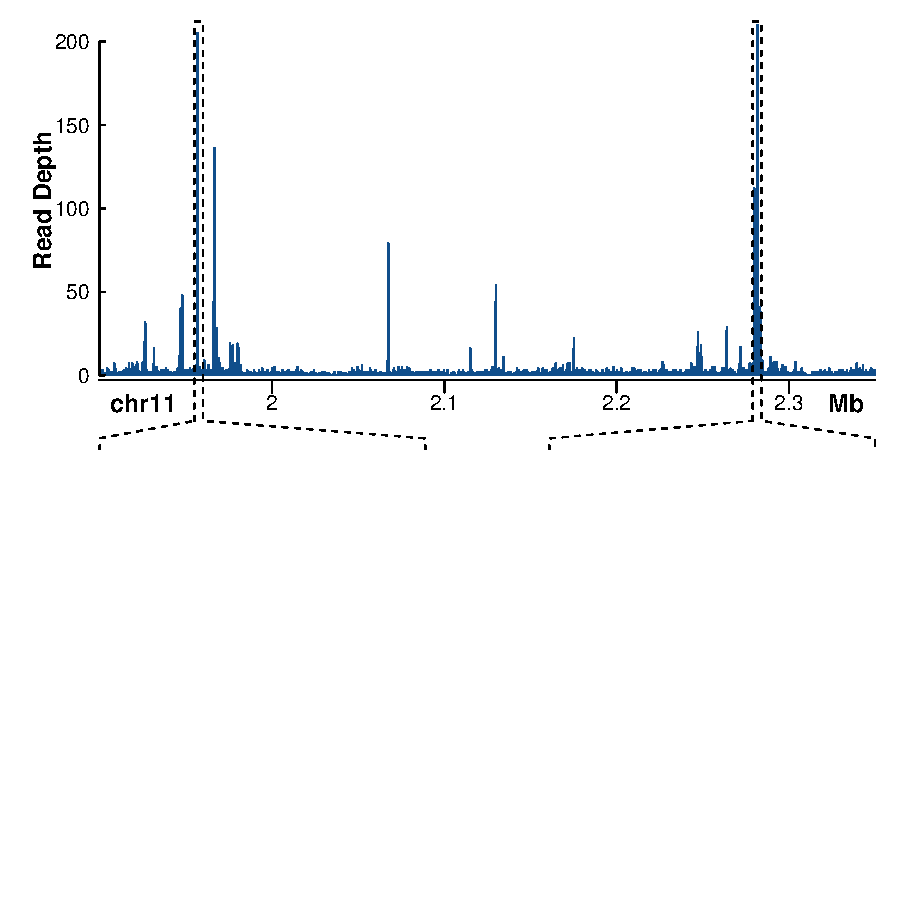
\includegraphics{Sushi-036}
\end{center}

Then we can add each of the zoomed inset regions.  For, each region we need execute the 'zoombox' function in order to draw the lines around the new plots.

\begin{Schunk}
\begin{Sinput}
> plotBedgraph(Sushi_DNaseI.bedgraph,chrom,chromstart=zoomregion1[1],
              chromend=zoomregion1[2])
> labelgenome(chrom,chromstart=zoomregion1[1],chromend=zoomregion1[2],
             n=4,scale="Kb",edgeblankfraction=0.2,cex.axis=.75)
> zoombox()
> mtext("Read Depth",side=2,line=1.75,cex=1,font=2)
> axis(side=2,las=2,tcl=.2)
> plotBedgraph(Sushi_DNaseI.bedgraph,chrom,chromstart=zoomregion2[1],
              chromend=zoomregion2[2])
> labelgenome(chrom,chromstart=zoomregion2[1],chromend=zoomregion2[2],
             n=4,scale="Kb",edgeblankfraction=0.2,cex.axis=.75)
> zoombox()
> mtext("Read Depth",side=2,line=1.75,cex=1,font=2)
> axis(side=2,las=2,tcl=.2)
\end{Sinput}
\end{Schunk}


\begin{center}
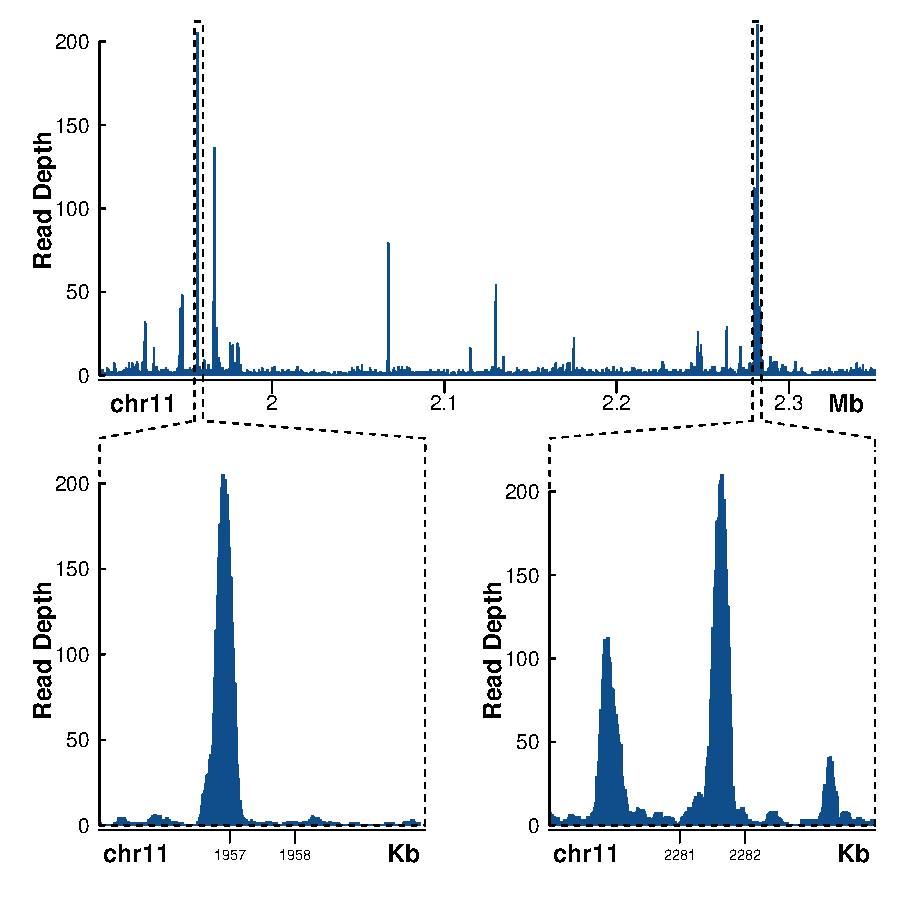
\includegraphics{Sushi-038}
\end{center}

\end{document}

